
\section{Next steps.}

The {\it e1-6} data is being processed at the moment of this writing.
All techniques presented above are going to be used (some are used already) for this period:

\begin{itemize}
\item Data reduction
\item Kinematic corrections
\item Acceptance calculation
\item Radiative correction
\end{itemize} 
After clean $\pi^0$ events are selected and corrected, the c.m. cross section 
$\Dfrac{d\sigma}{d\Omega^*_{\pi^0}}$ will be calculated.
Then for each $W$,$Q^2$,$cos\theta^*$ bin, a fit to the 
$\phi^*$ distributions similar to the one in Fig.\ref{fig:cross_fit} gives us the response functions 
$\sigma_L$, $\sigma_T$, $\sigma_{TT}$ and $\sigma_{LT}$ as a function of $W$, $Q^2$, $cos\,\theta^*$ as mentioned
in section 2.1.
\vspace{3.5 cm}
\begin{figure}[h]
 \begin{center} 
  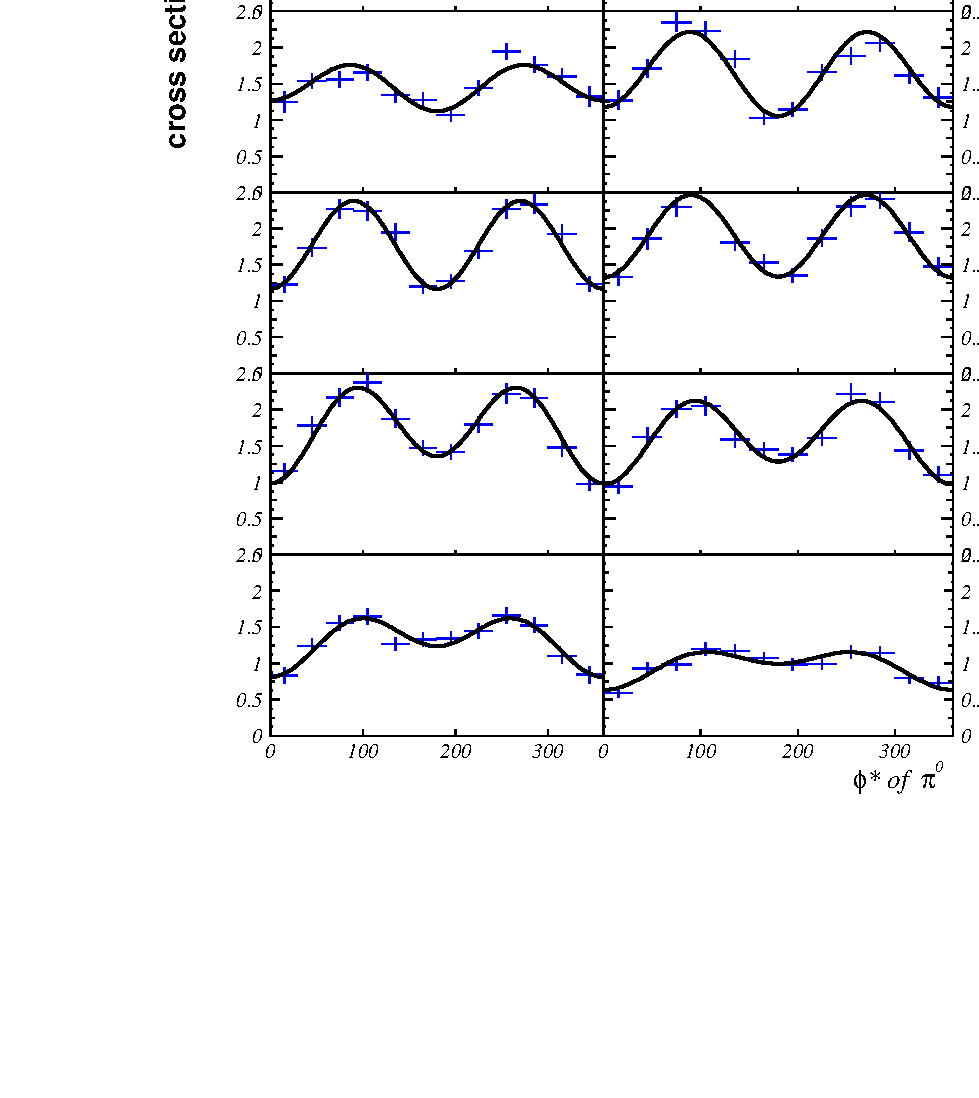
\includegraphics[height = 10cm, bb = 0 140 500 500]{img/cross_fit} 
  \caption{\cit Fits of $\phi$ distributions in CM for different $cos\theta^*$ bins. Data comes from {\rm e1c} run period.}
 \label{fig:cross_fit}
 \end{center}
\end{figure}

A fit of each response function with legendre polynomials in $cos\,\theta^*$ 
gives us the partial wave coefficients. For example, including
$l=0,1,2$ one has:
$$ 
\begin{array}{l c l}
\sigma_T + \epsilon\sigma_L & = & A_0 + A_1cos\theta^* + A_2P_2(cos\theta^*) + A_2P_3(cos\theta^*) + A_3P_4(cos\theta^*)\\
\sigma_{TT}  & = & B_0 + B_1cos\theta^* \\ 
\sigma_{LT} +  & = & C_0 + C_1cos\theta^* + C_2P_2(cos\theta^*) \\
\end{array}
$$
With the $M_{1+}$ dominance assumption discussed above, when $l$ goes only up to 1,  we simply have:
$$
\begin{array}{l c l}
| M_{1+} |^2 & = & A_0/2 \\
Re(E_{1+}M_{1+}) & = & (A_2 - 2B_0/3)/8 \\
\end{array}
$$



